\chapter{Introduzione al Software}

\section{Descrizione e Vincoli}

Il software sviluppato implementa un web service per la gestione delle prenotazioni di una sala prove.\newline
Lo sviluppo del software è iniziato definendo dei requisiti sull'orario della sala e sulla definizione delle richieste di prenotazione valide. In particolare:

\begin{itemize}
	\item La sala prove in questione offre 3 sale, prenotabili per turni di 2 ore e 30 minuti
	\item Ciascuna sala è prenotabile per qualunque orario (il minutaggio non deve necessariamente essere un multiplo di 30, la sala prove rimane aperta h24)
	\item È possibile effettuare una prenotazione fino a 5 minuti prima dell'orario specificato
	\item Tutte le prenotazioni richiedenti un'orario $o$, $o <= ora\ attuale\ +\ 5\ minuti$ vengono rifiutate
	\item Soltanto gli utenti registrati nel sistema possono effettuare le prenotazioni
	\item Le prenotazioni vengono associate in maniera univoca all'username scelto in fase di registrazione
	\item Non possono esistere due utenti con lo stesso username
\end{itemize}

\section{Panoramica del Software}

Il software è stato implementato utilizzando diverse tecniche di programmazione fra cui il \textsl{Test-Driven-Development}, \textsl{Build-Automation} (\textsl{Maven} e \textsl{Gradle}), \textsl{Continuous Integration}\dots seguendo una filosofia di sviluppo modulare. Possiamo dividere i vari pacchetti in pacchetti di \textbf{utilità} (model, exceptions, configurations\dots) e pacchetti di \textbf{servizio} (services, repository, web)

\begin{minipage}{\linewidth}
	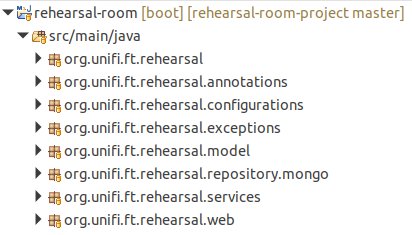
\includegraphics[width=\textwidth]{img/packages.png}
	\captionof{figure}{Gerarchia dei pacchetti}
\end{minipage}

L'applicazione è stata sviluppata utilizzando il \textsl{Framework Spring Boot}, grazie al quale è stata facilitata l'implementazione e la gestione di un database MongoDB (che consiste di due differenti repository: uno per gli utenti e uno per le prenotazioni) e l'esposizione dei metodi offerti dai vari \textsl{services} grazie ai Web Controller.\newline\newline
Le operazioni sui repository sono implementati appunto dalle classi contenute in $org.unifi.ft.rehearsal.services$: BandService e Scheduler.\newline
BandService si occupa della gestione della registrazione nel sistema dei gruppi che vogliono usufruire della sala prove. Le operazioni possibili sono il salvataggio di un utente nel sistema e la ricerca di un determinato utente tramite \textsl{username}.\newline
La classe Scheduler implementa invece le operazioni di salvataggio delle prenotazioni. Essendo questo servizio utilizzato dagli utenti sono fornite diverse operazioni per il salvataggio, la ricerca e la cancellazione.\newline\newline
Come accennato all'inizio del paragrafo, questi servizi sono esposti tramite un'interfaccia web realizzata grazie al \textsl{framework Model View Controller} offerto da \textsl{Spring Boot}, di cui verrà approfondito il funzionamento nei paragrafi successivi.